\let\negmedspace\undefined
\let\negthickspace\undefined
\documentclass[journal]{IEEEtran}
\usepackage[a5paper, margin=10mm, onecolumn]{geometry}
%\usepackage{lmodern} % Ensure lmodern is loaded for pdflatex
\usepackage{tfrupee} % Include tfrupee package

\setlength{\headheight}{1cm} % Set the height of the header box
\setlength{\headsep}{0mm}     % Set the distance between the header box and the top of the text

\usepackage{gvv-book}
\usepackage{gvv}
\usepackage{cite}
\usepackage{amsmath,amssymb,amsfonts,amsthm}
\usepackage{algorithmic}
\usepackage{graphicx}
\usepackage{textcomp}
\usepackage{xcolor}
\usepackage{txfonts}
\usepackage{listings}
\usepackage{enumitem}
\usepackage{mathtools}
\usepackage{gensymb}
\usepackage{comment}
\usepackage[breaklinks=true]{hyperref}
\usepackage{tkz-euclide} 
\usepackage{listings}
% \usepackage{gvv}                                        
\def\inputGnumericTable{}                                 
\usepackage[latin1]{inputenc}                                
\usepackage{color}                                            
\usepackage{array}                                            
\usepackage{longtable}                                       
\usepackage{calc}                                             
\usepackage{multirow}                                         
\usepackage{hhline}                                           
\usepackage{ifthen}                                           
\usepackage{lscape}
\begin{document}

\bibliographystyle{IEEEtran}
\vspace{3cm}

\title{AE - 2014}
\author{AI24BTECH11015 - Harshvardhan Patidar}
 \maketitle
% \newpage
% \bigskip
{\let\newpage\relax\maketitle}

\renewcommand{\thefigure}{\theenumi}
\renewcommand{\thetable}{\theenumi}
\setlength{\intextsep}{10pt} % Space between text and floats


\numberwithin{equation}{enumi}
\numberwithin{figure}{enumi}
\renewcommand{\thetable}{\theenumi}

\begin{enumerate}
    \item A student is required to demonstrate a high level of \underline{comprehension} of the subject, especially in the
    social sciences. \\ \\ The word closest in meaning to \underline{comprehension} is
        \begin{enumerate}
            \item understanding
            \item meaning
            \item concentration
            \item stability
        \end{enumerate}

    \item Choose the most appropriate word from the options given below to complete the following
    sentence. \\ \\ One of his biggest \_\_\_\_\_\_\_ was his ability to forgive.
        \begin{enumerate}
            \item vice
            \item virtues
            \item choices
            \item strength
        \end{enumerate}

    \item Rajan was not happy that Sajan decided to do the project on his own. On observing his unhappiness, Sajan explained to Rajan that he preferred to work independently. \\ \\ Which one of the statements below is logically valid and can be inferred from the above sentences?
        \begin{enumerate}
            \item Rajan has decided to work only in a group.
            \item Rajan and Sajan were formed into a group against their wishes.
            \item Sajan had decided to give in to Rajan's request to work with him.
            \item Rajan had believed that Sajan and he would be working together.
        \end{enumerate}
        
    \item If $y = 5x^2 +3$, then the tangent at $x=0, y=3$
        \begin{enumerate}
            \item passes through $x=0, y=0$
            \item has a slope of $+1$
            \item is parallel to the $x$-axis
            \item has a slope of $-1$
        \end{enumerate}

    \item A foundry has a fixed daily cost of Rs $50,000$ whenever it operates and a variable cost of Rs $800Q$, where $Q$ is the daily production in tonnes. What is the cost of production in Rs per tonne for a daily production of $100$ tonnes?
    
    \subsection*{Q.\ref{6} - Q.\ref{10} carry two marks each.}

    \item \label{6} Find the odd one in the following group: ALRVX, EPVZB, ITZDF, OYEIK
        \begin{enumerate}
            \item ALRVX
            \item EPVZB
            \item ITZDF
            \item OYEIK
        \end{enumerate}

    \item Anuj, Bhola, Chandan, Dilip, Eswar and Faisal live on different floors in a six-storeyed building (the ground floor is numbered $1$, the floor above it $2$, and so on). Anuj lives on an even-numbered floor. Bhola does not live on an odd numbered floor. Chandan does not live on any of the floors below Faisal's floor. Dilip does not live on floor number $2$. Eswar does not live on a floor immediately above or immediately below Bhola. Faisal lives three floors above Dilip. Which of the following floor-person combinations is correct?
    
        \begin{table}[h!]    
            \centering
                \begin{tabular}{|c|c|c|c|c|c|c|}
    \hline
    & Anuj & Bhola & Chandan & Dilip & Eswar & Faisal \\ \hline
    (A) & 6 & 2 & 5 & 1 & 3 & 4 \\ \hline
    (B) & 2 & 6 & 5 & 1 & 3 & 4 \\ \hline
    (C) & 4 & 2 & 6 & 3 & 1 & 5 \\ \hline
    (D) & 2 & 4 & 6 & 1 & 3 & 5 \\ \hline
    \end{tabular}
            \caption{}
            \label{7}
        \end{table}

    \item The smallest angle of a triangle is equal to two thirds of the smallest angle of a quadrilateral. The ratio between the angles of the quadrilateral is $3:4:5:6$. The largest angle of the triangle is twice its smallest angle. What is the sum, in degrees, of the second largest angle of the triangle and the largest angle of the quadrilateral?
    \item One percent of the people of country $X$ are taller than $6$ ft. Two percent of the people of country $Y$ are taller than $6$ ft. There are thrice as many people in country $X$ as in country $Y$. Taking both countries together, what is the percentage of people taller than $6$ ft?
        \begin{enumerate}
            \item $3.0$
            \item $2.5$
            \item $1.5$
            \item $1.25$
        \end{enumerate}

    \item \label{10} The monthly rainfall chart based on $50$ years of rainfall in Agra is shown in the following figure \ref{10fig}. Which of the following are true? ($k$ percentile is the value such that $k$ percent of the data fall below that value)
        \begin{figure}[H]
            \centering
            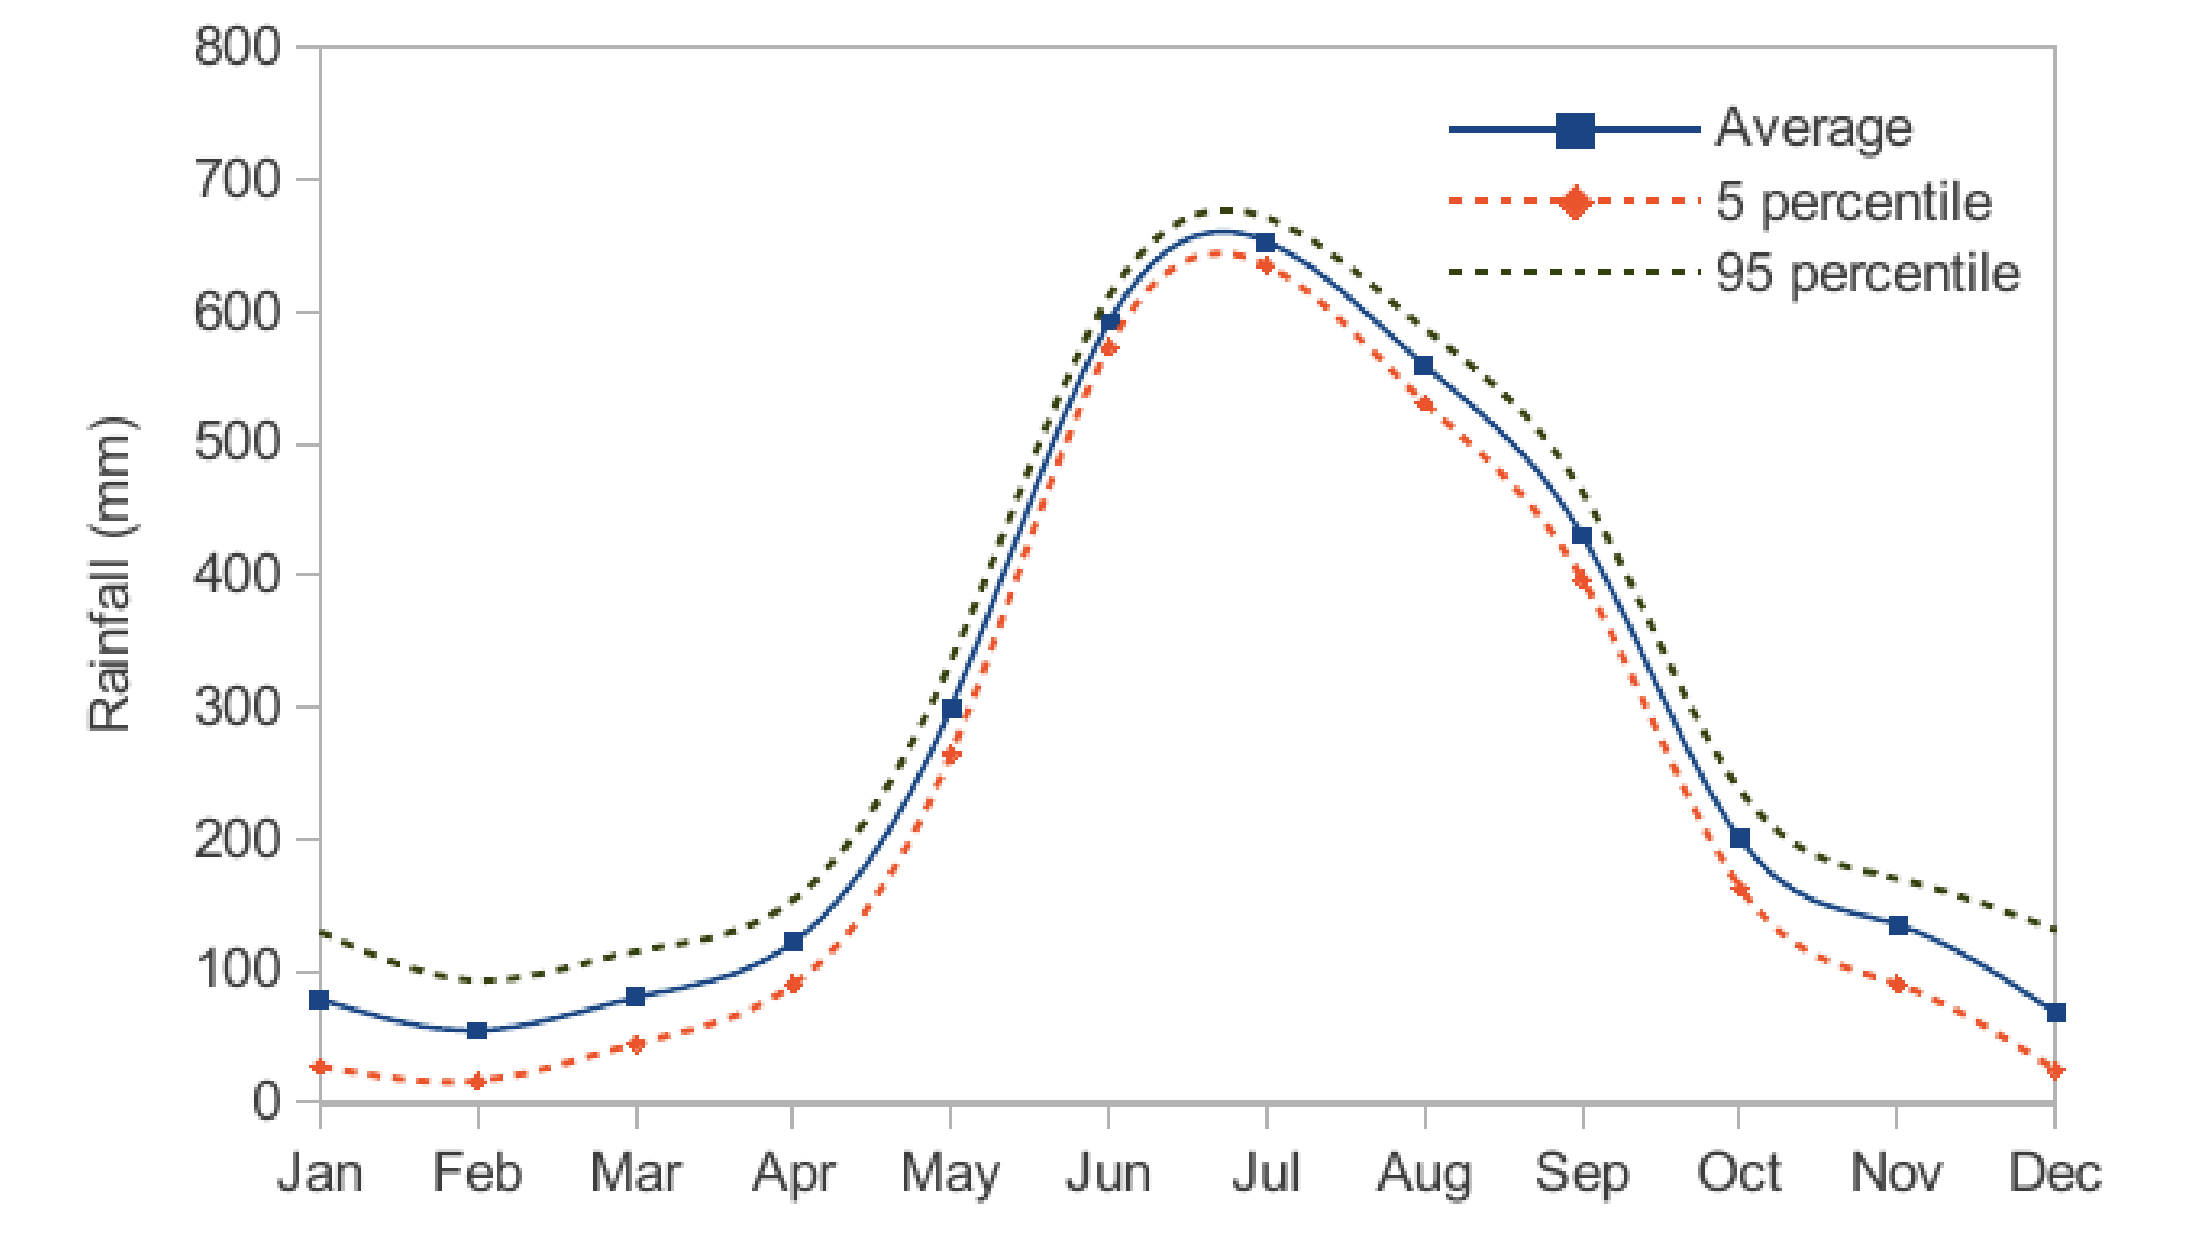
\includegraphics[width = 1\linewidth]{figs/10.png}
            \caption{}
            \label{10fig}
        \end{figure}

        \begin{itemize}
            \item[(i)] On average, it rains more in July than in December
            \item[(ii)] Every year, the amount of rainfall in August is more than that in January
            \item[(iii)] July rainfall can be estimated with better confidence than February rainfall
            \item[(iv)] In August, there is at least $500 mm$ of rainfall
        \end{itemize}

        \begin{enumerate}
            \item (i) and (ii)
            \item (i) and (iii)
            \item (ii) and (iii)
            \item (iii) and (iv)
        \end{enumerate} 

    \subsection*{Q.\ref{1a} - Q.25 carry one mark each.}
        \item \label{1a} For a real symmetric matrix $\sbrak{\vec{A}}$, which of the following statements is true:
            \begin{enumerate}
                \item The matrix is always diagonalizable and invertible.
                \item The matrix is always invertible but not necessarily diagonalizable.
                \item The matrix is always diagonalizable but not necessarily invertible.
                \item The matrix is always neither diagonalizable nor invertible.
            \end{enumerate}

        \item The series $s = \sum_{m=1}^{\infty} \frac{m^2}{3^m} \brak{x-2}^m$ converges for all $x$ with $\abs{x-2} \leq R$ given by 
            \begin{enumerate}
                \item $R=0$
                \item $R=3$
                \item $R=\infty$
                \item $R=\frac{1}{3}$
            \end{enumerate}

        \item The function given by $f\brak{x} = \begin{cases}  \sin \brak{1/x}, x \neq 0 \\ 0, x=0 \end{cases}$ is
            \begin{enumerate}
                \item Unbounded everywhere
                \item Bounded and continuous everywhere
                \item Bounded but not continuous at $x=0$
                \item Continous and differentiable everywhere
            \end{enumerate}
    \end{enumerate}

  
\end{document}


